\chapter{Installation and Configuration}

\section{Software requirements}

The \fmipp \trnsys FMU Export Utility is intended to run on Windows~7~(32-bit).

The following applications need to be installed prior to installing the \fmipp \trnsys FMU Export Utility:
\begin{itemize}
  \item \href{http://www.trnsys.com/}{\trnsys~17}
  \item \href{https://www.python.org/}{\python} (tested with \python~2.7)
  \item Microsoft Visual Studio Express 2013 for Windows Desktop
\end{itemize}


\section{Installation}
\label{sec:install}

To install the \fmipp \trnsys FMU Export Utility , proceed as follows:
\begin{itemize}
  \item Download the latest version as ZIP-file from the \href{http://sourceforge.net/projects/trnsys-fmu/files/latest/download}{download page}.
  \item Unzip the installation file into any sub directory (referred to as the \emph{installation directory}).
\end{itemize}

Installation requires to execute \python from the command prompt window, please refer to the \href{https://docs.python.org/2/faq/windows.html}{\python~FAQ} in case you need assistance with this.

Open the command prompt window, change to the installation directory and execute the script \texttt{trnsys\_fmu\_install.py}:
\begin{verbatim}
python.exe trnsys_fmu_install.py <trnsys_install_dir>
\end{verbatim}
where \texttt{<trnsys\_install\_dir>} is the path to your local \trnsys installation directory (typically \texttt{C:\symbol{92}Trnsys17}).

After successful installation, \type is available in the \trnsys Simulation Studio. An additional directory called \emph{FMI} should be available in the toolbar on the right-hand side, containing the new \trnsys type (\emph{\typea} and \emph{\typeb}), see Figure~\ref{fig:simulation_studio_overview} for a snapshot.

\begin{figure}
\centering{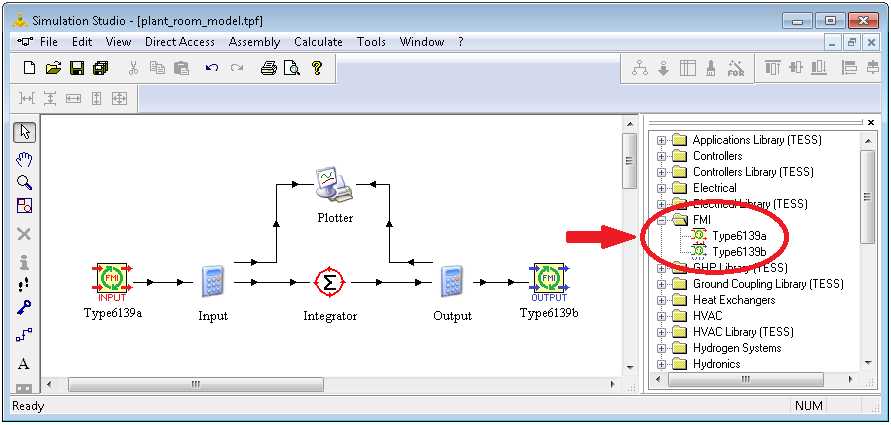
\includegraphics[width=\textwidth]{simulation_studio_overview}}
\caption{Simulation Studio with \type successfully installed.}
\label{fig:simulation_studio_overview}
\end{figure}
